\subsection{Comparison with recent related work}
Table~\ref{tab:recent-context} places the evaluation in the context of representative work published or released between 2024 and 2026. The table records the scale and selected findings reported by the respective authors, with particular attention to what each system verifies. Hardware, interaction models, cryptographic libraries, and security relations differ, so source-reported times cannot be converted into a common performance ranking.

\begin{table}[htbp]\centering\footnotesize
\caption{Selected quantitative findings from recent systems and the boundaries of comparison. Values are reported by the cited sources.}\label{tab:recent-context}
\begin{tabularx}{\linewidth}{@{}p{0.17\linewidth}p{0.24\linewidth}X@{}}\toprule
Method&Evaluation scale&Reported outcome and methodological boundary\\\midrule
BFT-PoLoc~\citep{BFTPoLoc} (2024)&Up to 450 challengers&At 450 challengers, roughly 45\% of localization uncertainty was below 100 km and 95\% below 1000 km; Byzantine network localization rather than a zero-knowledge policy proof\\
PG~\citep{PG} (2024)&261 cloud nodes; 19 constrained sensors&Private Byzantine-tolerant fusion using distributed garbled circuits, with an output-delivery guarantee\\
ZKLP~\citep{ZKLP} (2025)&Floating-point location SNARK&Proximity proof about 0.26 s and verification throughput about 470 peers/s; geometric properties of a hidden point\\
Vehicle ZK-PoL~\citep{VehiclePolicy} (2025)&Up to 43,800 trajectory points&Electric-vehicle subsidy and highway compliance proofs about 36 min and 59 min; interactive, trajectory-scale setting\\
CRSF~\citep{CRSF} (2026)&Up to 261 sensors&Approximately one second for the measured phases at the largest instance; collusion-resistant private fusion rather than a policy certificate\\\bottomrule
\end{tabularx}
\end{table}

To reduce differences attributable to hardware, we also reproduced a fixed version of the publicly available ZKLP implementation. ZKLP was pinned to commit \texttt{e8e321524982} and its first ZKLP32 test vector was executed on the same GitHub Actions Ubuntu runner as our $(n,d)=(3,2)$ subset circuit. Both use Groth16/BN254 and were measured over ten proof generations after setup. However, ZKLP depends on a branch based on gnark v0.9.1, whereas our implementation uses gnark v0.14.0, and the proved relations are different. This is therefore a comparison under a shared runner, not a fully controlled experiment with identical libraries and predicates.

\begin{table}[htbp]\centering\footnotesize
\caption{Fixed-version ZKLP reproduction and subset circuit on the same runner (sample medians over ten post-setup proofs).}\label{tab:zklp-repro}
\setlength{\tabcolsep}{3pt}
\begin{tabularx}{\linewidth}{@{}Xrrrrr@{}}\toprule
Implementation&Constraints&Prove (ms)&Verify (ms)&Proof (B)&Public witness (B)\\\midrule
Pinned ZKLP32&19,467&515.53&1.739&196&140\\
Our subset $(3,2)$&32,474&645.14&1.547&164&556\\\bottomrule
\end{tabularx}
\end{table}

ZKLP mainly proves geometric predicates of a hidden coordinate. Our corresponding circuit additionally checks three signed uncertainty intervals, issuer roster and context constraints, threshold support, and a four-valued classification. Its larger circuit and public witness therefore include additional authentication work; their difference cannot be attributed exclusively to geometric-algorithm efficiency. An older \texttt{m6i.xlarge} record in the ZKLP repository reports 21,878 constraints and 270.03 ms median proving time, while the pinned code compiles to 19,467 constraints in the current environment. The records alone do not isolate the effects of version, hardware, or configuration, and we do not interpret the difference as a performance trend.

\subsection{Cryptographic performance and circuit scalability}
\subsubsection{Structural reference using a simplified relation}
Table~\ref{tab:point-zk} reports a hidden-point region-membership circuit on the same cryptographic stack. It contains only a test of whether a private point belongs to the public policy; it omits issuer signatures, interval uncertainty, Byzantine budgets, threshold fusion, and four-valued output. It is therefore a reference for the cost of a weaker relation, not a functionally matched baseline.

\begin{table}[htbp]\centering\small
\caption{Simplified hidden-point membership circuit with 16-bit bounds under Groth16/BN254.}\label{tab:point-zk}
\begin{tabular}{rrrr}\toprule
Dimension $d$&R1CS constraints&Proof (B)&Public witness (B)\\\midrule
2&408&164&268\\
3&612&164&396\\\bottomrule
\end{tabular}
\end{table}

By contrast, the smallest complete subset circuits contain 32,474 constraints at $(n,d)=(3,2)$ and 35,248 at $(3,3)$. Their additional constraints arise jointly from in-circuit signature verification, issuer-key and coordinate checks, context binding, threshold fusion, and the four-valued relation. They cannot all be attributed to robust geometry alone. In each tested configuration, a Groth16 proof occupies 164 bytes.

\subsubsection{Measured costs of the two geometric backends}
Tables~\ref{tab:crypto} and~\ref{tab:subset} report lower-corner and threshold-subset costs for matched small configurations. Each circuit is set up once and evaluated using 30 proofs. Figure~\ref{fig:scaling} displays the distribution of proving times. Public witness sizes span 556--748 bytes across the reported shapes, excluding report plaintext and transport framing.

\begin{table}[htbp]\centering\small
\caption{Lower-corner Groth16 measurements. Setup is in seconds; all other times are in milliseconds.}\label{tab:crypto}
\begin{tabular}{rrrrrrr}\toprule
$(n,d)$&Constraints&Setup&Prove p50&Prove p95&Verify p50&Verify p95\\\midrule
$(3,2)$&55,987&3.64&213.12&244.83&1.033&1.350\\
$(4,2)$&97,493&7.47&360.74&427.17&1.081&1.514\\
$(5,2)$&158,781&11.56&574.69&700.49&1.073&1.212\\
$(3,3)$&185,229&13.84&548.33&707.35&1.067&1.412\\
$(4,3)$&510,362&38.34&1090.95&1212.54&1.093&1.506\\\bottomrule
\end{tabular}
\end{table}

\begin{table}[htbp]\centering\small
\caption{Threshold-subset Groth16 measurements for $k=n-1$ (times in milliseconds).}\label{tab:subset}
\begin{tabular}{rrrr}\toprule
$(n,d)$&Constraints&Prove p50&Verify p50\\\midrule
$(3,2)$&32,474&163.42&1.028\\
$(4,2)$&42,918&225.79&1.038\\
$(5,2)$&53,528&254.66&1.051\\
$(3,3)$&35,248&206.34&1.059\\
$(4,3)$&46,737&234.93&1.038\\\bottomrule
\end{tabular}
\end{table}

\begin{figure}[htbp]\centering
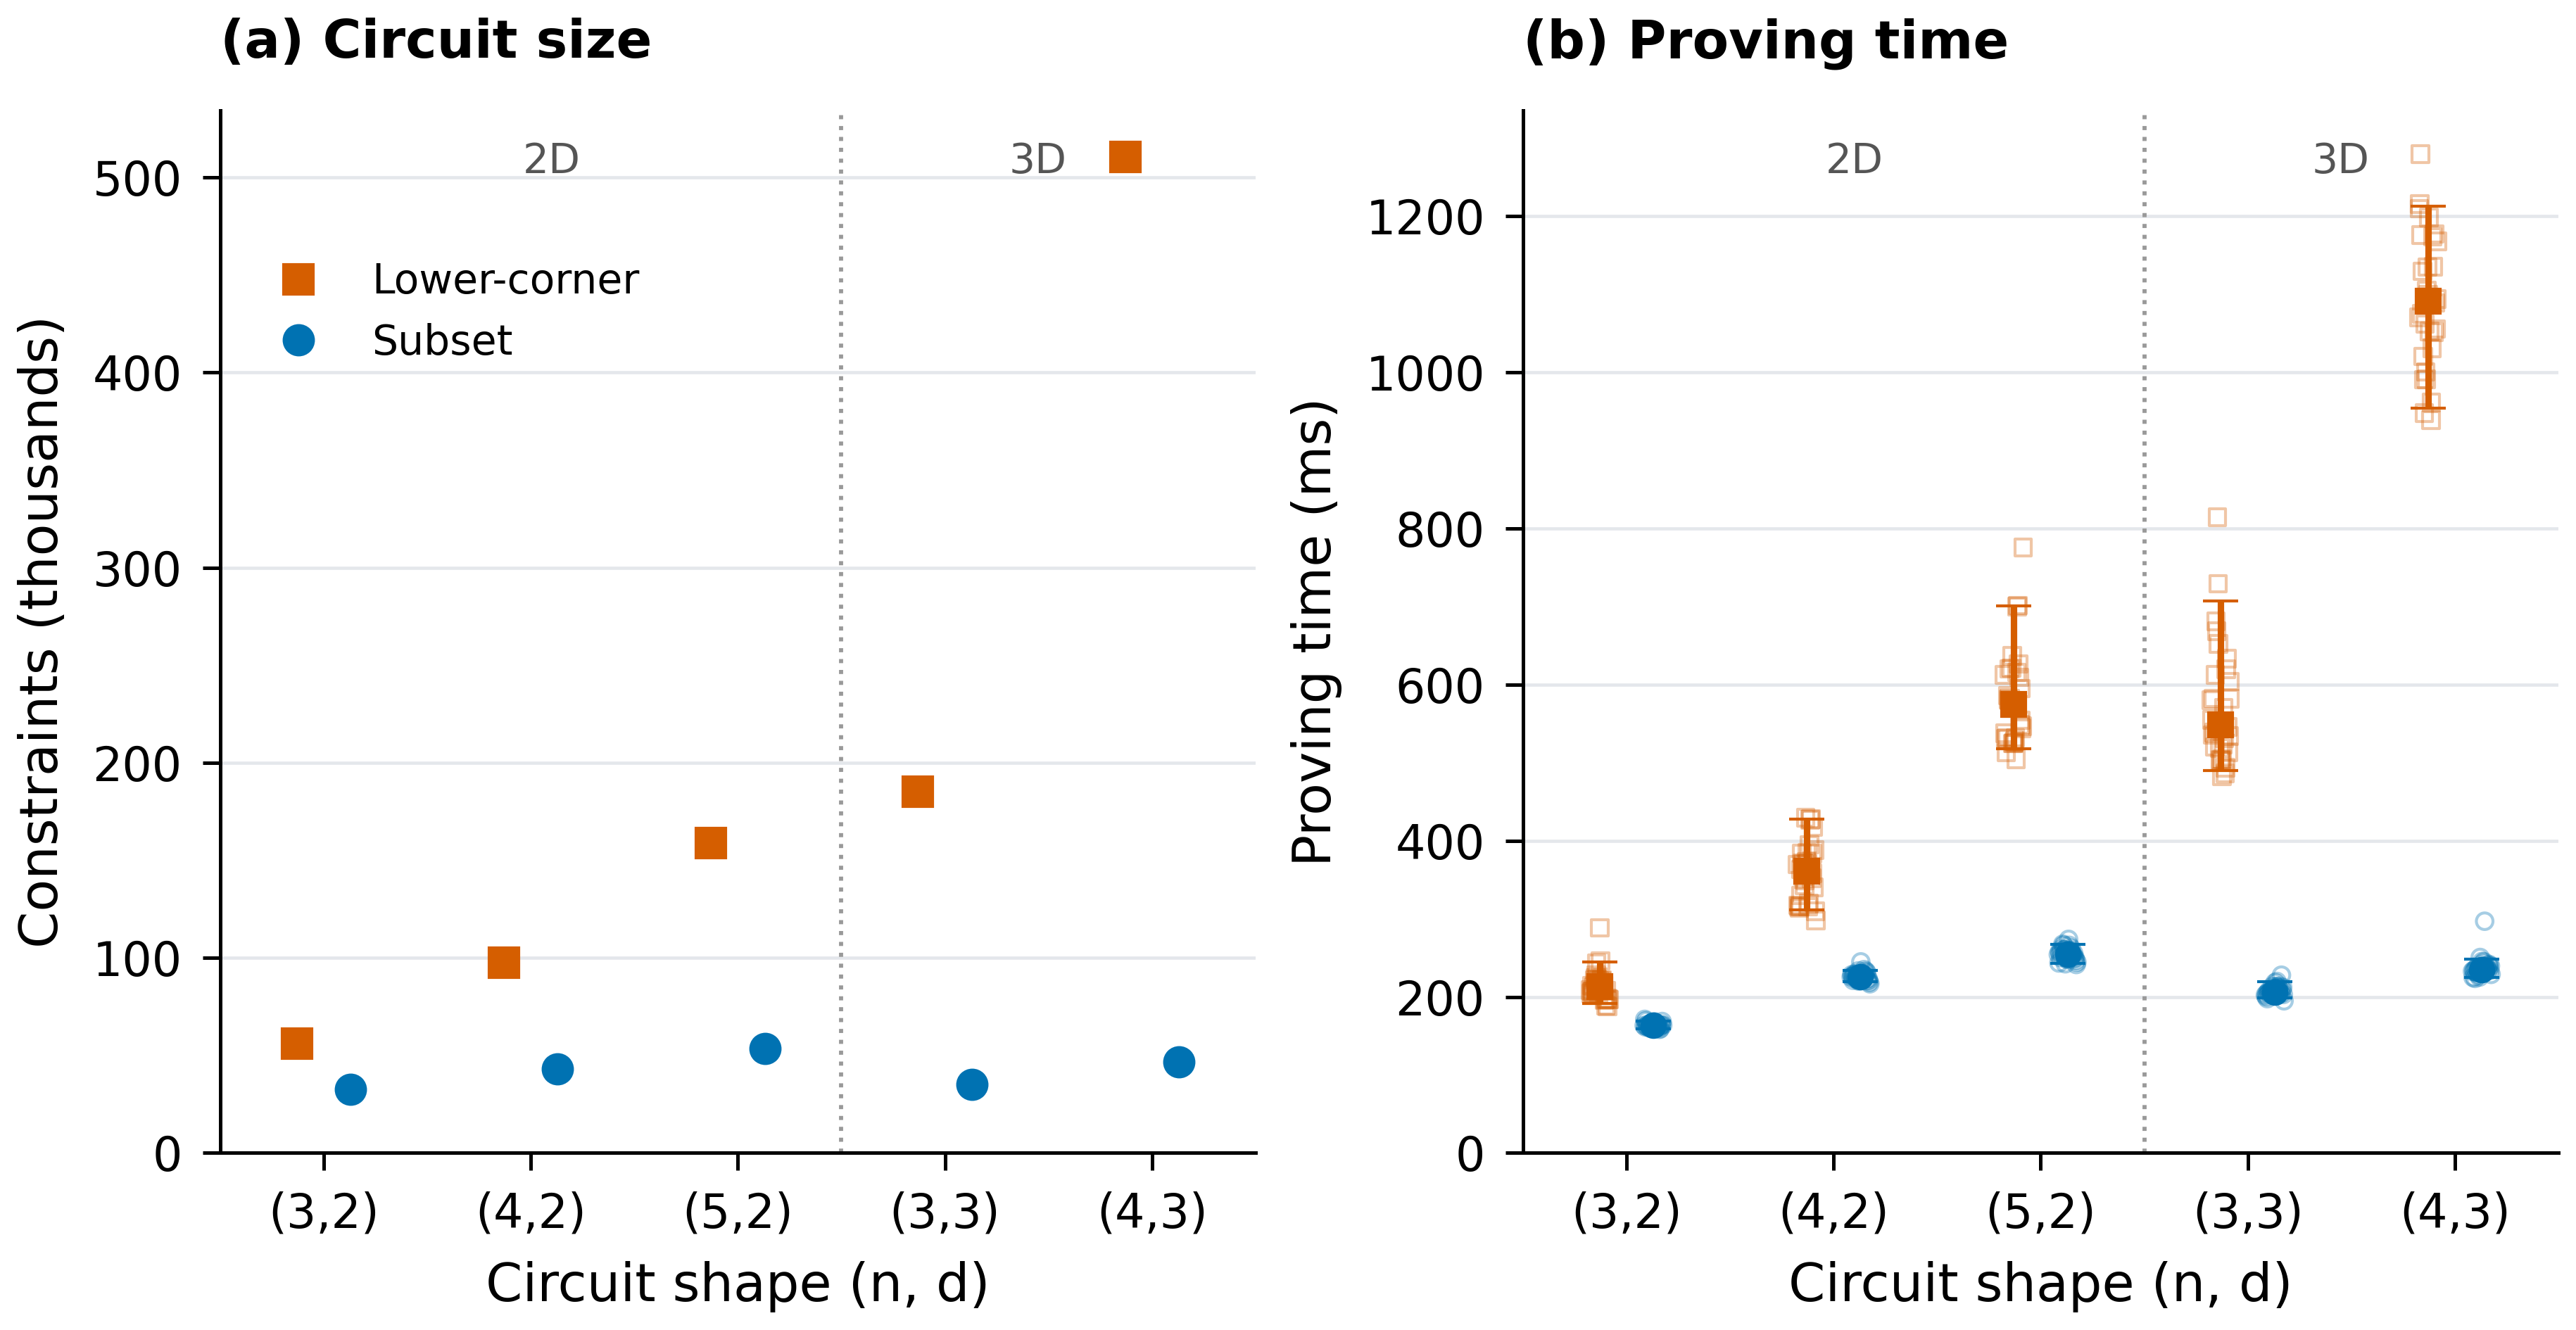
\includegraphics[width=\linewidth]{backend_costs.png}
\caption{R1CS size and proving time for the two backends on the Apple M1 platform. Small points in the timing panel show all 30 observations per circuit shape and backend (300 total); large markers are medians and intervals span the empirical p5--p95 range, not confidence intervals. Backend batches were not interleaved.}\label{fig:scaling}
\end{figure}

Subset enumeration has fewer constraints in every tested configuration with $k=n-1$. For example, at $(n,d)=(4,3)$, lower-corner reachability requires 510,362 constraints and has a median proving time of 1090.95 ms; the subset backend requires 46,737 constraints and 234.93 ms. The observed ratio of approximately 4.64 is descriptive for the specified test platform, because the backend batches were not interleaved. It is not a universal speedup corrected for environmental variation, and smaller circuits do not by themselves establish the same advantage at every size.

\subsubsection{Resource-limited compilation scalability}
Figure~\ref{fig:compilegrowth} and Table~\ref{tab:compilegrowth} summarize 32 resource-bounded compilation invocations. Of these, 27 completed; five were terminated after the sampled RSS reached the 3 GiB threshold, indicated by \texttt{RL}. At $(d,n)=(2,16)$, lower-corner reachability has 3,509,645 constraints, compared with 181,194 and 308,978 constraints for subsets with omissions $b=n-k$ equal to one and two. At $(d,n,k)=(3,12,6)$, the balanced-threshold subset circuit already has 962,018 constraints. We do not assign estimated counts to unfinished builds or claim that they are theoretically uncomputable.

\begin{table}[htbp]\centering\small
\caption{Resource-limited R1CS compilation sweep with complete signature and geometric constraints. \texttt{RL} indicates termination before a count was obtained.}\label{tab:compilegrowth}
\begin{tabular}{rrrrrr}\toprule
$d$&$n$&Lower corner&Subset $b=1$&Subset $b=2$&Subset $k=n/2$\\\midrule
2&4&97,493&42,918&43,160&43,160\\
2&8&509,277&86,354&97,734&111,776\\
2&12&1,544,390&132,447&181,221&675,759\\
2&16&3,509,645&181,194&308,978&RL\\
3&4&510,362&46,737&47,099&47,099\\
3&8&RL&95,153&112,213&133,255\\
3&12&RL&147,506&220,640&962,018\\
3&16&RL&203,793&395,417&RL\\\bottomrule
\end{tabular}\end{table}

\begin{figure}[htbp]\centering
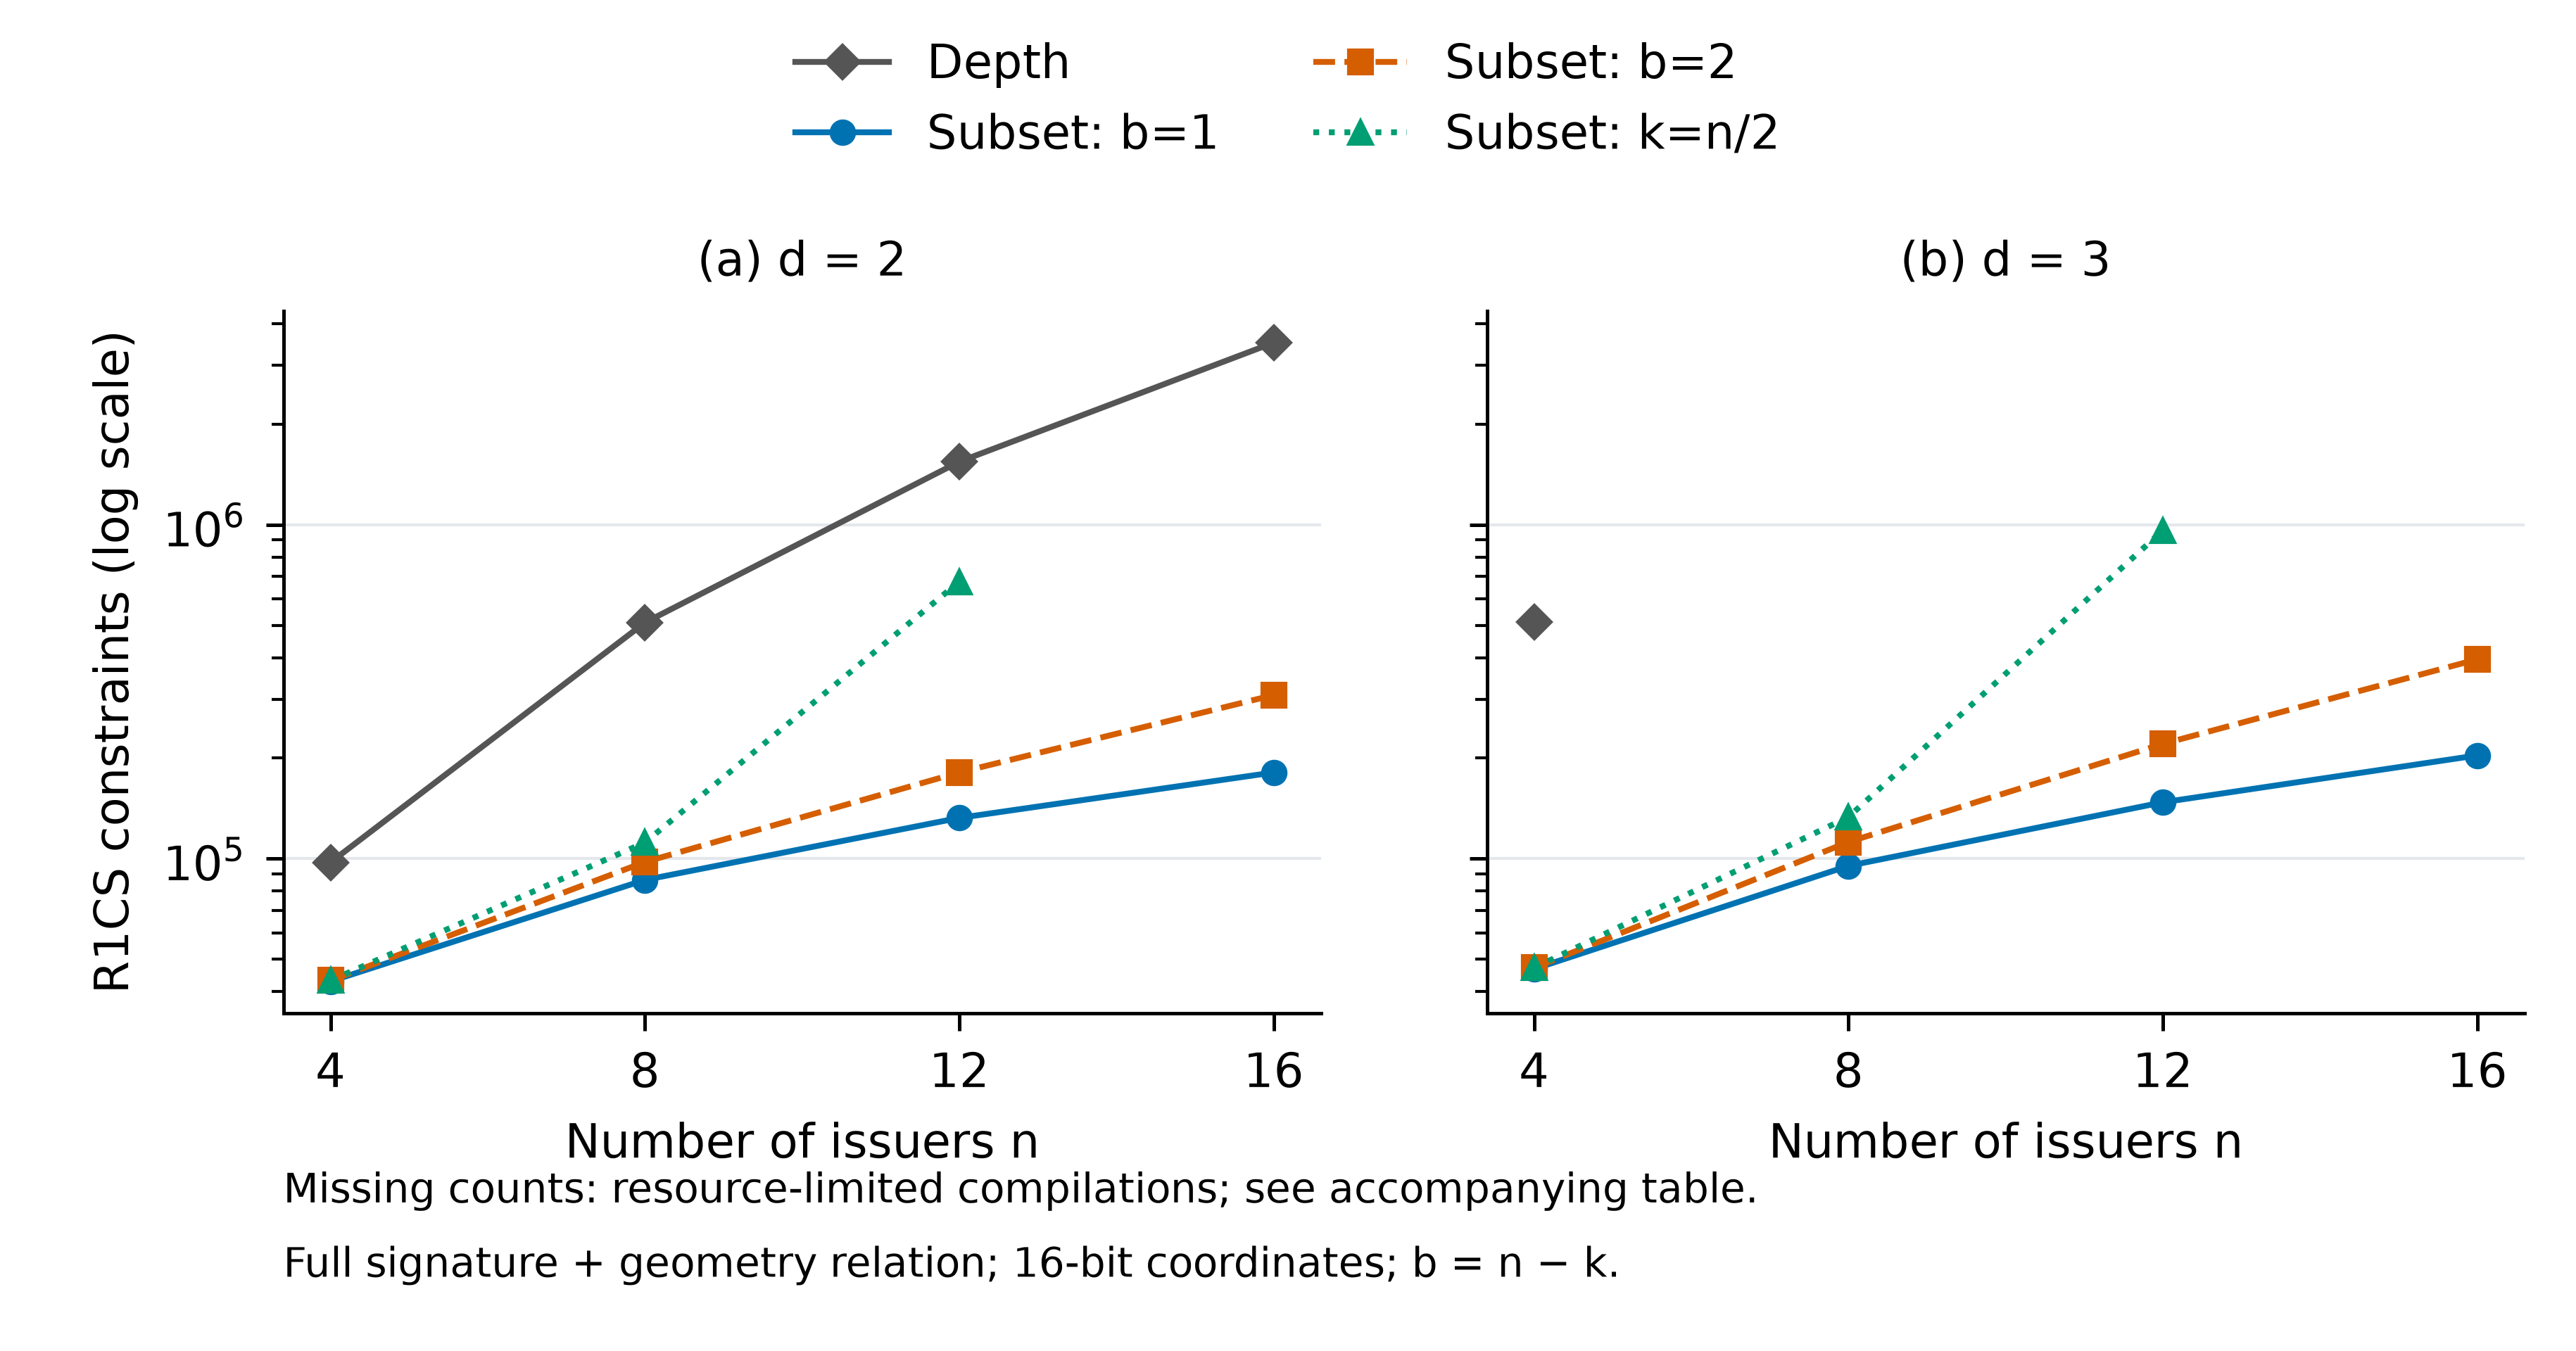
\includegraphics[width=\linewidth]{compile_scalability.png}
\caption{Resource-limited sweep of full R1CS constraint counts. Missing markers correspond to terminated compilations, not zero constraints; connecting lines are visual guides. These are compilation results, not large-circuit proving times.}\label{fig:compilegrowth}
\end{figure}

Taken together, the direct measurements and compilation results favor subset enumeration for the tested small omission budgets $b=f+r$. As $k$ approaches half the source count, however, the number of subsets $\binom nk$ grows rapidly and can diminish the advantage. The evidence supports backend selection for particular tested scales and thresholds, rather than a universal optimum across dimensions, source populations, and hardware.
